\FILE{Cloudmask.tex}

\subsection{MLCommons Cloudmask Workflow}
\label{cloudmask-workflow}

Cloudmask is a program that develops a model to classify sections of
satellite images as either containing clouds or clear sky by using
machine learning. This is beneficial for temperature measurement and
meteorology.  Information regarding Cloudmask can be found on its
GitHub page~\cite{www-cloudmask}.  One of our goals is to run
Cloudmask for benchmarking.  As benchmarking Cloudmask requires
several phases and scripts, including a mixture of shell scripts and
Python scripts, leveraging Cloudmesh-cc provides a much easier runtime
instead of manually issuing many commands at a terminal.  We have
created a sample workflow the runs a coordinated workflow across a
number of hybrid resources. This includes an HPC computer at
University of Virginia called Rivanna, as well as two desktop
computers. This workflow can easily be adapted to include other machines. In this
particular workflow, we execute the benchmarks on a number of
different CUDA cards (see Figure~\ref{fig:cloudmaskwf}. For Rivanna,
the code also utilizes our cloudmesh-vpn component that provides the
ability to connect to the UVA VPN from Python, then fetches the data
and executes the various benchmarks once the data is available.

\begin{figure*}[htb]
\centering
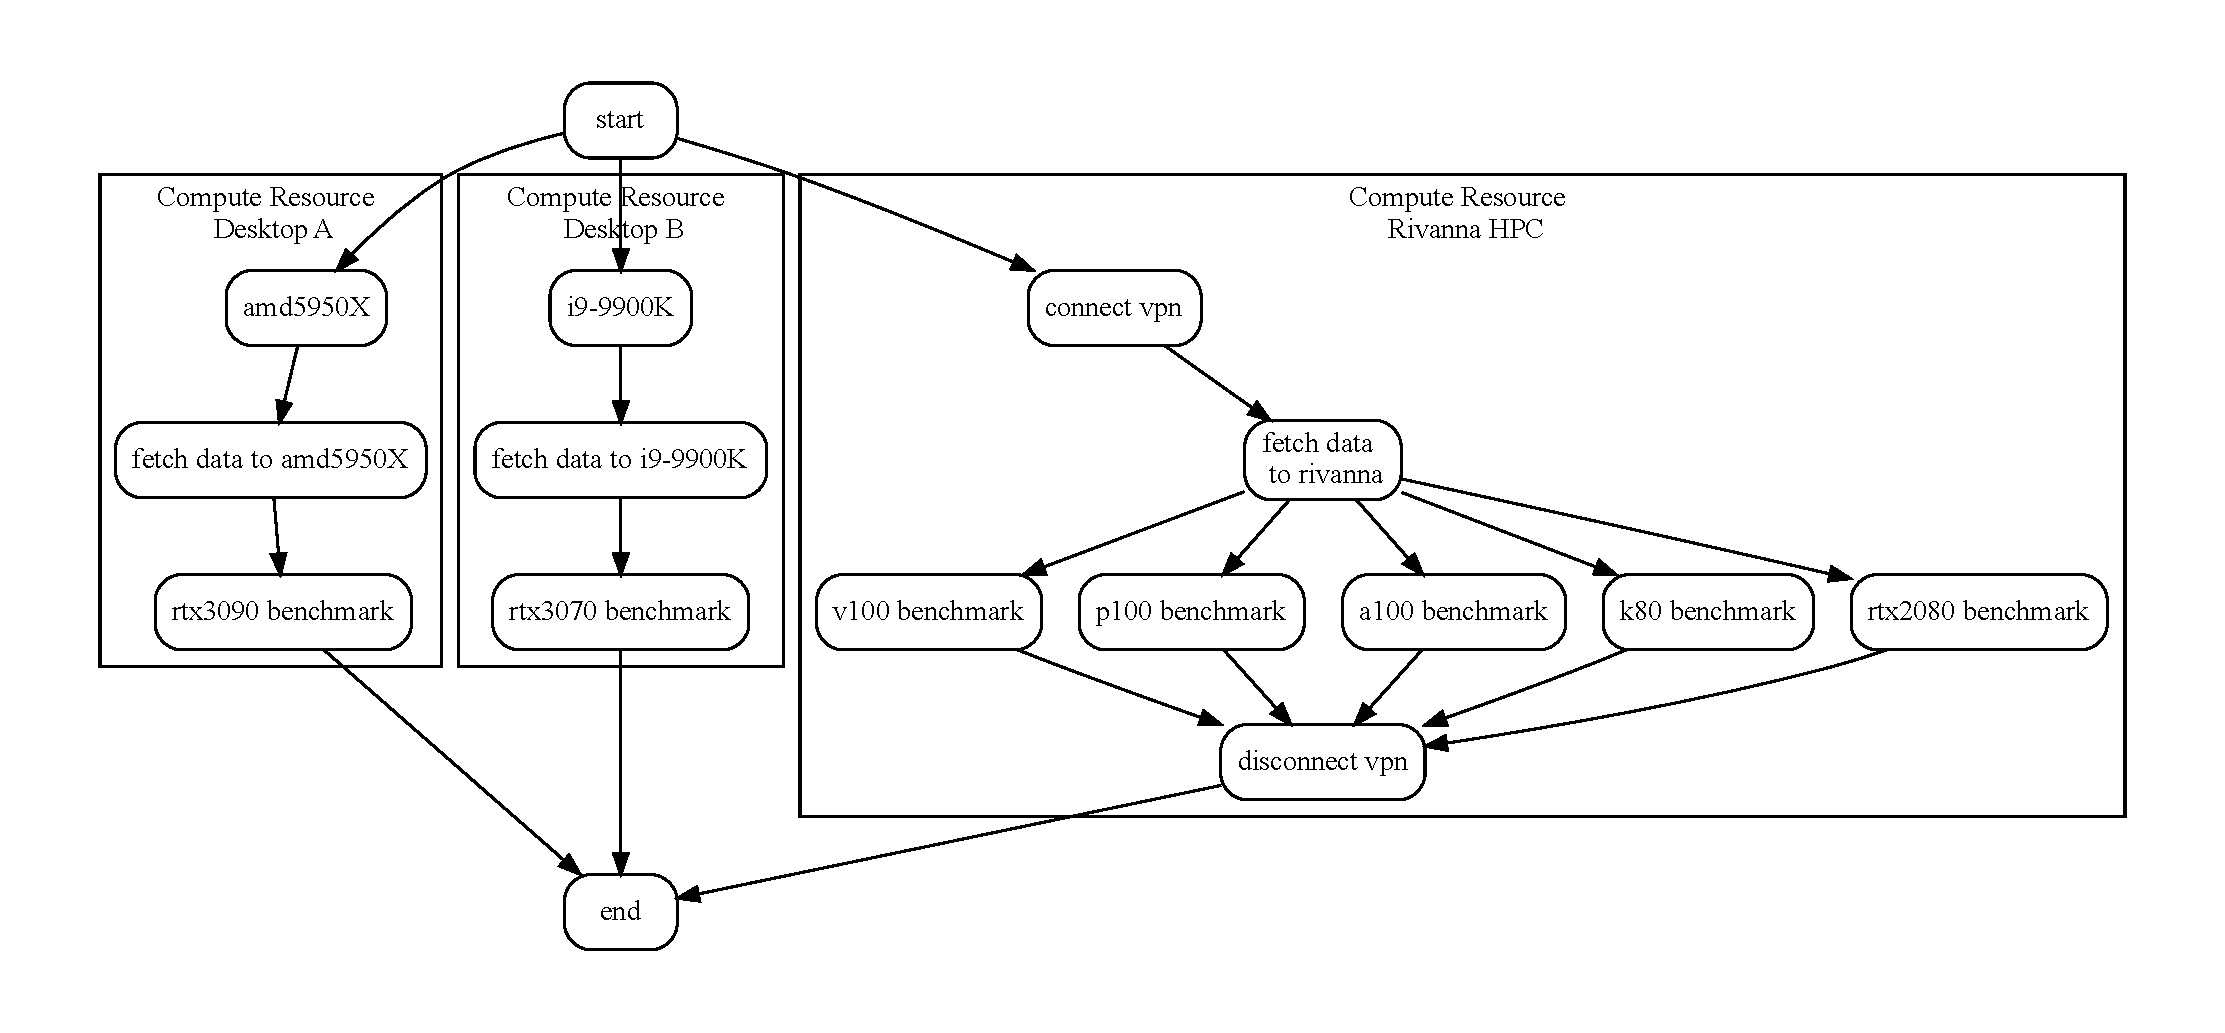
\includegraphics[width=0.75\textwidth]{images/cloudmask-wf.pdf}
%\vspace{-1cm}
\caption{Workflow for Cloudmask}\label{fig:cloudmaskwf}
\end{figure*}

The workflow will take approximately 24 hours to run if resources are
available. The workflow iterates through the five GPUs available on
Rivanna, including V100, P100, A100, K80, and RTX2080, and runs the program
three times on each GPU. Each run trains the model with 10, 30, and 50
epochs for benchmarking. Upon completing a run, the logs and
benchmarks are written into a results folder.
In the appendix we showcase just how to run a portion of this workflow
while utilizing only Rivanna (see Appendix~\ref{sec:running-cloudmask}).


